\documentclass{beamer} 
% \documentclass[compress]{beamer} %makes things tighter
% \documentclass[handout]{beamer} %to make handouts (aka remove pauses)
\usepackage{amsmath, graphics, graphicx, tabularx, algorithm, algorithmic, appendixnumberbeamer, siunitx, multicol, tikz}
\usetikzlibrary{arrows, automata}

\tikzset{
  invisible/.style={opacity=0},
  visible on/.style={alt={#1{}{invisible}}},
  alt/.code args={<#1>#2#3}{%
    \alt<#1>{\pgfkeysalso{#2}}{\pgfkeysalso{#3}} % \pgfkeysalso doesn't change the path
  },
}

\let\Tiny=\tiny % this gets rid of that super annoying font warning

\graphicspath{{../Talk-imgs/}}


%%%%%%%%%%%%%%%%%%%%%%%%%%%%%%%%%%%%%%
%% THEME DEFINITION %%%%%%%%%%%%%%%%%%
%%%%%%%%%%%%%%%%%%%%%%%%%%%%%%%%%%%%%%

% \usetheme{Warsaw} %bulkier but more informative header, if too big can use compress
\usetheme{Frankfurt} %if even with compress is too ugly, then this is a nicer minimal header

% this removes the navigation buttons on each slide
\setbeamertemplate{navigation symbols}{}

% this changes the footer to add the date and slide numbers
\setbeamertemplate{footline}
{
  \leavevmode%
  \hbox{%
  \begin{beamercolorbox}[wd=.25\paperwidth,ht=2.25ex,dp=1ex,center]{author in head/foot}% this is the normal first box with the author name
    \usebeamerfont{author in head/foot}\insertshortauthor
  \end{beamercolorbox}%
  \begin{beamercolorbox}[wd=.60\paperwidth,ht=2.25ex,dp=1ex,center]{title in head/foot}% I changed this box to also include the date
    \usebeamerfont{title in head/foot}\insertshorttitle
  \end{beamercolorbox}%
  \begin{beamercolorbox}[wd=.15\paperwidth,ht=2.25ex,dp=1ex,center]{slide num in head/foot}% I created this box to have the slide counter
    \insertframenumber{} / \inserttotalframenumber
  \end{beamercolorbox}
  }%
  \vskip0pt%
}
% \setbeamercolor{slide num in head/foot}{fg=white, bg=black} % Warsaw theme: change the color to match the first box
\setbeamercolor{slide num in head/foot}{fg=white, bg=structure.fg} %if using Frankfurt theme, use this color definition


%%%%%%%%%%%%%%%%%%%%%%%%%%%%%%%%%%%%
%% METHOD FOR CITING ON SLIDE%%%%%%%
%%%%%%%%%%%%%%%%%%%%%%%%%%%%%%%%%%%%
\usepackage[absolute,overlay]{textpos}

\setbeamercolor{framesource}{fg=black} % can do something like black!XX to make it (100-XX)% white for shades of gray
\setbeamerfont{framesource}{size=\tiny}

\newcommand{\source}[1]{
  \begin{textblock*}{\textwidth}(1.8cm,8.6cm)
    \begin{beamercolorbox}[ht=0.5cm,right]{framesource}
     \usebeamerfont{framesource}\usebeamercolor[fg]{framesource} {#1}
   \end{beamercolorbox}
  \end{textblock*}
}


%%%%%%%%%%%%%%%%%%%%%%%%%%%%%%%%%
%% set title, author etc %%%%%%%%
%%%%%%%%%%%%%%%%%%%%%%%%%%%%%%%%%

% format is \item[short]{long}
\title[Path optimization in free energy calculations]{Path optimization in alchemical free energy calculations}
\author{Ryan Muraglia\inst{1}}
\date{July 19, 2016}
% \subtitle{CBB preliminary examination}
\institute{\inst{1} Program in Computational Biology \& Bioinformatics\\Duke University}


%%%%%%%%%%%%%%%%%%%%%%%%%%%%%%%
%% BEGIN DOCUMENT %%%%%%%%%%%%%
%%%%%%%%%%%%%%%%%%%%%%%%%%%%%%%
\begin{document}

% Title slide
\frame{ \titlepage }

% Initial outline
\frame{ 
  \frametitle{Outline}
  \tableofcontents
}

\frame{
  \frametitle{Modulating binding in biological systems}
  \begin{columns}
  \column{0.5\textwidth}
  \begin{block}{Rational molecular design}
  \begin{itemize} 
  \setlength{\itemsep}{1pt}
  \setlength{\parskip}{0pt}
  \setlength{\parsep}{0pt}
  \item Free energy of binding determines behavior of system
  \item Changes to the ligands affect the free energy
  \item Predict change in free energy for a given set of ligand mutations
  \item Select mutations with desired properties (enhance or destabilize binding)
  \end{itemize}
  \end{block}
  \column{0.6\textwidth}
  \begin{figure}
  \centering
  \includegraphics[scale=0.5]{bnab2.jpg} 
  \end{figure}
  \end{columns}
  \source{P.D. Kwong, J.R. Mascola, G.J. Nabel, \emph{Nat. Rev. Immunol.} \textbf{13}, 693 (2013)}
}

\section[FEC primer]{Free energy calculation primer}

\frame{
  \frametitle{A probabilistic representation of molecules}
  \begin{columns}
  \column{0.8\textwidth}
  \begin{itemize}
  \item Atomic coordinates: $r \equiv \{\boldsymbol{r_1}, ..., \boldsymbol{r_N}\}$
  \item Atomic momenta: $p \equiv \{\boldsymbol{p_1}, ..., \boldsymbol{p_N}\}$
  \item State representation: $x \equiv \{ r, p\}$
  \item Kinetic energy: $K(p) = \sum_{i=1}^N \frac{p_i^2}{2m_i}$
  \item Potential energy: $U(r) = U_{bond} + U_{angle} + U_{dihedral} + U_{elec} + U_{vdW}$
  \item Hamiltonian: $H(x) = K(p) + U(r)$
  \item Boltzmann weight: $q(x) = \exp(-\beta H(x))$
  \item Partition function: $Z=\int_\Omega \exp(-\beta H(x)) dx$
  \item Probability of state: $p(x) = q(x)/Z$
  \item Free energy: $G=-\beta^{-1}\log(Z)$
  \end{itemize}
  \column{0.2\textwidth}
  \vspace{-2ex}
  \begin{figure}
  \centering
  \includegraphics[scale=0.17]{Bond_stretching_energy.png} \\ \smallskip
  \includegraphics[scale=0.12]{Protein_backbone.png} 
  % \includegraphics[scale=0.1]{talk-images/LennardJones.png}
  \end{figure}
  \end{columns}
  \source{Wikimedia Commons}
}

\frame{
  \frametitle{The thermodynamic cycle}
  \begin{columns}
  \column{0.4\textwidth}
  Free energy differences can be expressed in terms of the ratio of partition functions:
  \begin{align*}
  \Delta G_{bind} &= G_{B} - G_{U} \\
                  &= -\beta^{-1}\log(Z_{B}/Z_{U})
  \end{align*}
  Many valid combinations of partition functions are accessible via a thermodynamic cycle.
  \column{0.6\textwidth}
  \vspace{-2ex}
  \begin{figure}
  \centering
  \includegraphics[scale=0.75]{thermcycle-cropped.jpg}
  \end{figure}
  \vspace{2ex}
  \end{columns}
  \source{J.D. Durrant, J.A. McCammon, \emph{BMC Biol.} \textbf{9}, 71 (2011)}
}

\frame{
  \frametitle{Exponential averaging and alchemical intermediates}
  \begin{columns}
  \column{0.3\textwidth}
  \begin{figure}
  \centering
  \includegraphics[scale=0.2]{alchemical-int.png}
  \end{figure}
  \column{0.8\textwidth}
  \begin{itemize}
  \item Exponential averaging (EXP) estimator: $\Delta G_{0 \rightarrow 1} = -\beta^{-1} \log E_0[\exp(-\beta(U_1(x)-U_0(x))]$
  \item Common problem: as the overlap between $p_0$ and $p_1$ decreases, the accuracy of the estimator deteriorates.
  \pause
  \item Solution: construct intermediate states, divide and conquer. \\ $\Delta G_{0 \rightarrow 1} = -\beta^{-1} \log \left( \frac{Z_1}{Z_{0.5}} \frac{Z_{0.5}}{Z_0}\right)$
  \end{itemize}
  \begin{block}{$\lambda$ scaling}
  \centering
  Define intermediate states with the potential:\\
  $U(\lambda) = \lambda U_1 + (1-\lambda) U_0$
  \end{block}
  \end{columns}
  \source{J.D. Durrant, J.A. McCammon, \emph{BMC Biol.} \textbf{9}, 71 (2011)}
}

\frame{
  \frametitle{Bridge sampling estimators}
  The Bennett acceptance ratio (BAR) method is part of the broader class of bridge sampling estimators, commonly used to estimate ratios of normalizing constants.

  \begin{block}{The bridge sampling identity}
  \begin{equation*}
  r \equiv \exp(-\beta\Delta G) = \frac{Z_1}{Z_0} = \frac{E_0[q_1(x)\alpha(x)]}{E_1[q_0(x)\alpha(x)]}
  \end{equation*}
  \end{block}

  This can be approximated by Monte Carlo integration: 

  \begin{block}{The bridge sampling estimator}
  \begin{equation*}
  \hat{r}=\frac{\frac{1}{n_0}\sum_{j=1}^{n_0}q_1(x_{0j})\alpha(x_{0j})}{\frac{1}{n_1}\sum_{j=1}^{n_1}q_0(x_{1j})\alpha(x_{1j})}
  \end{equation*}
  \end{block}
  where $\{x_{i1}, ..., x_{in}\}$ are draws from $p_i$, $i=0,1$.
}

\frame{
  \frametitle{The BAR estimator}
  \begin{block}{BAR's $\alpha$ function}
  \begin{equation*}
  \alpha \propto (s_1q_1+s_0rq_0)^{-1}
  \end{equation*}
  \end{block}
  where $s_i=n_i/(n_0+n_1)$. \\ \medskip
  % BAR is defined by the choice: $\alpha \propto (s_1q_1+s_2rq_2)^{-1}$, where $s_i=n_i/(n_1+n_2)$. \\

  This $\alpha$ minimizes the asymptotic variance of $\log(\hat{r})$.
  % The aymptotic optimality of BAR is guaranteed, as its derivation ensures that the asymptotic variance of $\log(\hat{r})$ is minimized.

  \begin{block}{The iterative BAR estimator}
  \begin{equation*}
  \hat{r}^{(t+1)} = \frac{ \frac{1}{n_0} \sum_{j=1}^{n_0} \left [ \frac{l_{0j}}{s_1 l_{0j} + s_0 \hat{r}^{(t)}} \right ]}{\frac{1}{n_1} \sum_{j=1}^{n_1} \left [ \frac{1}{s_1 l_{1j} + s_0 \hat{r}^{(t)}} \right ]}
  \end{equation*}
  \end{block}
  where $l_{ij}=q_1(x_{ij})/q_0(x_{ij})$, $j=1,...,n_i$, $i=0,1$
}

\frame{ 
  \frametitle{Outline}
  \tableofcontents
}

\section{Proof of concept}

\subsection{Gelman and Meng's result}

\frame{
  \frametitle{Optimal bridging densities}
  % For free energy calculations of interest, low phase space overlap is guaranteed: a sequence of alchemical intermediates will be used.

  \begin{block}{$\lambda$ scaling}
  \centering
  Define intermediate distributions with the potential: \\ $U(\lambda) = \lambda U_1 + (1-\lambda) U_0$
  \end{block}
  
  Selecting an appropriate number and placement of intermediates can have a profound effect on the free energy estimation.
  % \pause

  \begin{columns}
  \column{0.3\textwidth}
  \begin{figure}
  \centering
  \vspace{-2ex}
  \includegraphics[scale=0.32]{pathsampling.jpg}
  \end{figure}
  \column{0.3\textwidth}
  \begin{figure}
  \centering
  \vspace{-2ex}
  \includegraphics[scale=0.4]{pathsampling3.jpg}
  \end{figure}
  \column{0.2\textwidth}
  \begin{tiny}
  \begin{enumerate}
  \item Importance sampling
  \item Geometric bridge sampling
  \item Optimal bridge sampling
  % \item Geometric path sampling
  % \item Optimal path sampling in $\mu$ space
  % \item Optimal path sampling in $(\mu, \sigma)$ space
  \end{enumerate}
  \end{tiny}
  \end{columns}
  \source{A. Gelman, X.L. Meng, \emph{Stat. Sci.} \textbf{13}, 163 (1998)}
}

\subsection{Defining the augmented $\lambda$ space}

\frame{
  \setbeamercolor{alerted text}{fg=gray!50}
  \frametitle{Defining the expanded $\lambda$ space}
  Numerous options for expansion of $\lambda$ space: 
  \begin{itemize}
  \item \alert<2>{Separation of energy terms (Jiang \& Roux, 2010)
  \begin{itemize} \item $U(\lambda_{vdW}, \lambda_{elec}) = U_0 + U_{vdW}(\lambda_{vdW}) + U_{elec}(\lambda_{elec})$ \end{itemize} }
  \item \alert<2>{Addition of biasing potential (Darve et al., 2008)}
  \item Addition of temperature ladder (Sugita et al., 2000)
  \end{itemize} 
  \pause
  % General, non-specific boosting axis, applicable to any molecular system, doesn't depend on system specific knowledge like biasing potential
  \begin{block}{Temperature-augmented $\lambda$ space}
  \begin{itemize}
  \item Predictable benefits, analogous to REMD, conceptually similar to Gelman and Meng's optimal path
  \item Potential energy is unaffected: $U(x, \lambda)=\lambda U_1(x) + (1-\lambda) U_0(x)$
  \item Temperature changes Boltzmann weights: $q(x, \lambda, \beta) = \exp(-\beta U(x, \lambda))$
  \end{itemize}
  \end{block}
}

\subsection{Exhaustive search}

\frame{
  \frametitle{Exhaustive search I - G\&M in discrete space}
  \begin{figure}
  \centering
  \includegraphics[scale=0.3]{unimod-3pan-searchv2.png}
  \end{figure}
  %note: sigma=sqrt(T), distance metric=totvar dist
}

\frame{
  \frametitle{Exhaustive search II - Generalized to other distributions}
  \begin{figure}
  \centering
  \includegraphics[scale=0.3]{unib1-3pan-searchv1.png}
  \end{figure}
}

\frame{
  \frametitle{Exhaustive search III - Cost-adjusted varBAR}
  \begin{block}{Asymptotic variance of the BAR estimator}
  \scalebox{1.1}{
    $\text{var}(\widehat{\Delta G}) = \frac{1}{N}\left [ \left \langle \frac{1}{2+2\cosh(\widehat{\Delta G} - \Delta U(x) -M)} \right \rangle ^{-1}- \left ( \frac{N}{N_0} + \frac{N}{N_1} \right ) \right ]
    $}
  \end{block}
  \begin{columns}
  \column{0.8\textwidth}
  \begin{figure}
  \centering
  \includegraphics[scale=0.325]{kshortest.png}
  \end{figure}
  \column{0.3\textwidth}
  \begin{table}
  \centering
  \begin{tabular}{c|c}
   & Left \\ \hline
  Aug & 3.18E-4 \\
  Std & 5.07E-4
  \end{tabular}

  \begin{tabular}{c|c} \hline \hline
   & Right \\ \hline
  Aug & 5.93E-5 \\
  Std & 7.03E-5
  \end{tabular}
  \end{table}
  \end{columns}
}

\section[SMC for path traversal]{Sequential Monte Carlo for path traversal}

\frame{
  \frametitle{Two sides of path optimization}
  \begin{itemize}
    \item Up to now, we've been focused on optimizing the reaction coordinate - the constituent states of the alchemical path.
    \item The manner in which we traverse a given path represents a complementary side to path optimization.
    \item To obtain $n$ draws for a path with $k$ states, each with a relaxation time of $\tau$, would require $\mathcal{O}(\tau k n)$ computation with equilibrium sampling.
    \item A sequential sampler with transition cost $\tau^\prime$, where $\tau >> \tau^\prime$ can accomplish the equivalent task in $\mathcal{O}((\tau + (k-1)\tau^\prime)n)$ time, representing a significant cost reduction.
  \end{itemize}
}

\frame{
  \frametitle{Graphical representation of (non)equilibrium samplers}
  \begin{figure}
  \centering
  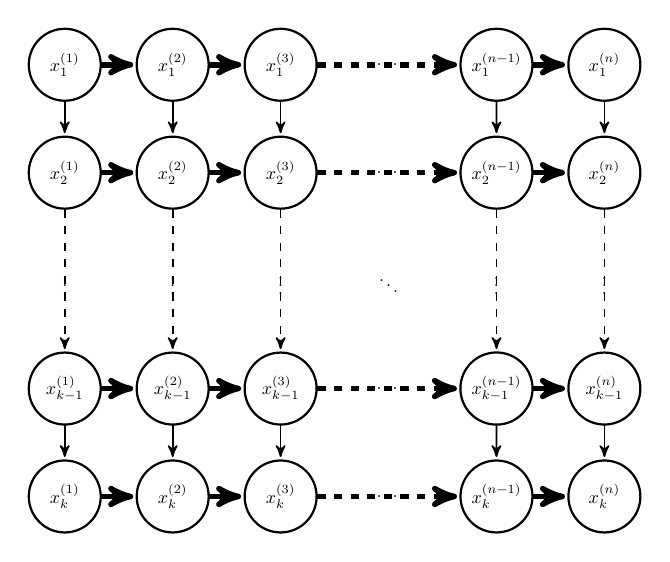
\begin{tikzpicture}[->,>=stealth',shorten >=1pt, auto, node distance=6em, semithick]
  \tikzstyle{every state}=[fill=white,draw=black,thick,text=black, scale=0.65,minimum size=4em]
  \node[state] (x11) {$x_1^{(1)}$};
  \node[state] (x12) [right of=x11] {$x_1^{(2)}$};
  \node[state] (x13) [right of=x12] {$x_1^{(3)}$};
  \node[state] (x1.) [right of=x13, draw=none] {$\dots$};
  \node[state] (x1-) [right of=x1.] {$x_1^{(n-1)}$};
  \node[state] (x1n) [right of=x1-] {$x_1^{(n)}$};
  \node[state] (x21) [below of=x11] {$x_2^{(1)}$};
  \node[state] (x22) [right of=x21] {$x_2^{(2)}$};
  \node[state] (x23) [right of=x22] {$x_2^{(3)}$};
  \node[state] (x2.) [right of=x23, draw=none] {$\dots$};
  \node[state] (x2-) [right of=x2.] {$x_2^{(n-1)}$};
  \node[state] (x2n) [right of=x2-] {$x_2^{(n)}$};
  \node[state] (x.1) [below of=x21, draw=none] {$\vdots$};
  \node[state] (x.2) [right of=x.1, draw=none] {$\vdots$};
  \node[state] (x.3) [right of=x.2, draw=none] {$\vdots$};
  \node[state] (x..) [right of=x.3, draw=none] {$\ddots$};
  \node[state] (x.-) [right of=x.., draw=none] {$\vdots$};
  \node[state] (x.n) [right of=x.-, draw=none] {$\vdots$};
  \node[state] (xk-1) [below of=x.1] {$x_{k-1}^{(1)}$};
  \node[state] (xk-2) [right of=xk-1] {$x_{k-1}^{(2)}$};
  \node[state] (xk-3) [right of=xk-2] {$x_{k-1}^{(3)}$};
  \node[state] (xk-.) [right of=xk-3, draw=none] {$\dots$};
  \node[state] (xk--) [right of=xk-.] {$x_{k-1}^{(n-1)}$};
  \node[state] (xk-n) [right of=xk--] {$x_{k-1}^{(n)}$};
  \node[state] (xk1) [below of=xk-1] {$x_k^{(1)}$};
  \node[state] (xk2) [right of=xk1] {$x_k^{(2)}$};
  \node[state] (xk3) [right of=xk2] {$x_k^{(3)}$};
  \node[state] (xk.) [right of=xk3, draw=none] {$\dots$};
  \node[state] (xk-) [right of=xk.] {$x_k^{(n-1)}$};
  \node[state] (xkn) [right of=xk-] {$x_k^{(n)}$};
  \path[line width=2.0pt] (x11) edge (x12);
  \path[line width=2.0pt] (x12) edge (x13);
  \path[line width=2.0pt] (x1-) edge (x1n);
  \path[line width=2.0pt, visible on=<1>] (x21) edge (x22);
  \path[line width=2.0pt, visible on=<1>] (x22) edge (x23);
  \path[line width=2.0pt, visible on=<1>] (x2-) edge (x2n);
  \path[line width=2.0pt, visible on=<1>] (xk-1) edge (xk-2);
  \path[line width=2.0pt, visible on=<1>] (xk-2) edge (xk-3);
  \path[line width=2.0pt, visible on=<1>] (xk--) edge (xk-n);
  \path[line width=2.0pt, visible on=<1>] (xk1) edge (xk2);
  \path[line width=2.0pt, visible on=<1>] (xk2) edge (xk3);
  \path[line width=2.0pt, visible on=<1>] (xk-) edge (xkn);
  \path[line width=2.0pt, dashed] (x13) edge (x1-);
  \path[line width=2.0pt, dashed, visible on=<1>] (x23) edge (x2-);
  \path[line width=2.0pt, dashed, visible on=<1>] (xk-3) edge (xk--);
  \path[line width=2.0pt, dashed, visible on=<1>] (xk3) edge (xk-);
  \path[visible on=<2>] (x11) edge (x21);
  \path[visible on=<2>] (x12) edge (x22);
  \path[visible on=<2>] (x13) edge (x23);
  \path[visible on=<2>] (x1-) edge (x2-);
  \path[visible on=<2>] (x1n) edge (x2n);
  \path[visible on=<2>] (xk-1) edge (xk1);
  \path[visible on=<2>] (xk-2) edge (xk2);
  \path[visible on=<2>] (xk-3) edge (xk3);
  \path[visible on=<2>] (xk--) edge (xk-);
  \path[visible on=<2>] (xk-n) edge (xkn);
  \path[visible on=<2>, dashed] (x21) edge (xk-1);
  \path[visible on=<2>, dashed] (x22) edge (xk-2);
  \path[visible on=<2>, dashed] (x23) edge (xk-3);
  \path[visible on=<2>, dashed] (x2-) edge (xk--);
  \path[visible on=<2>, dashed] (x2n) edge (xk-n);
  \end{tikzpicture}
  \end{figure}
}

\frame{
  \frametitle{Analogous SMC estimators}
  The $k$-th distribution can be approximated as: $p_k \sim w_k x_k$, where $w_k$ is the normalized incremental weight, given by $\tilde{w}_k = q_k(x_{k-1})/q_{k-1}(x_{k-1})$ for an MCMC transition kernel.
  \begin{block}{AIS - Annealed importance sampling}
  \begin{equation*} 
  \hat{r} = E_{0 \rightarrow 1}[\exp(-\beta w_1)]
  \end{equation*}
  \end{block}
  \begin{block}{CFT - Crooks fluctuation theorem}
  \begin{equation*}
  % \hat{r} = \frac{E_{0 \rightarrow 1}[w_1 q_1(x) \alpha(x)]}{E_{1 \rightarrow 0}[w_0 q_0(x) \alpha(x)]}
  \hat{r} = \frac{E_{0 \rightarrow 1}[(1+\exp(\beta w_1 + C))^{-1}]}{E_{1 \rightarrow 0}[(1+\exp(\beta w_0 - C))^{-1}]}
  \end{equation*}
  \end{block}
}

\subsection{Path sensitivity for SMC}

\frame{
  \frametitle{SMC methods are sensitive to path choice}
  \begin{figure}
  \centering
  \includegraphics[scale=0.4]{ais-pathcompare.jpg}
  \end{figure}
}

\subsection{Path selection and the multi-armed bandit}

\frame{
  \frametitle{Adaptive sample allocation}
  To efficiently select a best path when their qualities are not known \emph{a priori}, 
  sample usage must be partitioned between two conflicting tasks:
  \begin{itemize}
    \item Exploration of poorly characterized paths
    \item Exploitation of the putative optimal path
  \end{itemize}

  \pause
  \begin{block}{The multi-armed bandit problem}
  Given $k$ non-overlapping paths of unknown variance and $N$ particles with which to sample, what is the optimal sample allocation strategy that will minimize the variance of the overall free energy estimate?
  \end{block}
}

\frame{
  \frametitle{Comparison of simple bandit strategies}
  \begin{columns}
  \column{0.5\textwidth}
  \begin{figure}
  \centering
  \includegraphics[scale=0.55]{ais-bandit.png}
  \end{figure}
  \column{0.5\textwidth}
  \begin{itemize}
    \item \underline{Equal:} allocate particles equally to paths, regardless of estimated variances
    \item \underline{Greedy:} after initial equal allocation learning period, allocate all particles to best-guess minimum variance path
    \item \underline{Proptnl:} after initial equal allocation learning period, allocate particles to paths inversely proportional to their estimated variances
  \end{itemize}
  \end{columns}
}

\section{Full grid optimization}

\subsection{pCrooks -  a new estimator}

\frame{
  \frametitle{Limitations of SMC and the bandit framework}
  % A primary shortcoming of the bandit strategies is their reliance on fully defined paths. 
  The multi armed bandit is a suitable formulation when selecting between enumerated paths, but situations can arise where we have no preconceived notion of the underlying state space, and what an acceptable path looks like.

  A method that encompasses path discovery, refinement and selection is a necessity for more general applications.

  Because SMC estimators operate on full paths, they are not well suited to contexts in which we build paths edge-by-edge.
   % with SMC methods requires the development of a new SMC estimator

}

\frame{
  \frametitle{Edgewise decomposable SMC estimators}
  \begin{block}{seqBAR - sequential BAR}
  Approximate equilibrium distributions by resampling: redraw $n$ particles from the multinomial distribution where the probabilities are the particle weights. 

  Use resampled, unweighted particles in BAR equation.
  \end{block}

  \begin{block}{pCrooks - pairwise Crooks}
  Use per-transition work-weighted distributions in a modified BAR equation:
  \begin{equation*}\hat{r}_{A \rightarrow B} = \frac{E_{A \rightarrow B}[w_B q_B(x) \alpha(x)]}{E_{B \rightarrow A}[w_A q_A(x) \alpha(x)]}\end{equation*}
  \end{block}
}

\frame{
  \frametitle{SMC excels when paired with bridge sampling}
  \begin{figure}
  \centering
  \includegraphics[scale=0.5]{seqBARvAIS-uni-bi-v02.png}
  \end{figure}
}

\frame{
  \frametitle{pCrooks is the more robust edgewise SMC method}
  \begin{figure}
  \centering
  \includegraphics[scale=0.45]{pcrooks.jpg}
  \end{figure}
}

\subsection{Q-learning}

\frame{
  \frametitle{The Q-learning algorithm}
  Q-learning is a reinforcement learning technique for maximizing total reward in finite state Markov decision processes.

  Q-learning accomplishes this by estimation of a $Q$ function, which describes the expected reward for all state-action pairs in the graph.

  \begin{block}{$Q$-function updates}
  \begin{equation*}
  Q_{t+1}(s,a) = Q_t(s,a) + \alpha (R(s,a) + \gamma \max_{a^\prime}Q_t(s^{\prime}, a^{\prime}) - Q_t(s,a))
  \end{equation*}
  $\alpha \in [0,1]$ is a learning rate, and $\gamma \in [0,1]$ is a discount factor.
  \end{block}
}

\frame{
  \frametitle{The Q-learning algorithm}
  Q-learning is a reinforcement learning technique for maximizing total reward in finite state Markov decision processes.

  Q-learning accomplishes this by estimation of a $Q$ function, which describes the expected reward for all state-action pairs in the graph.

  \begin{block}{$Q$-function updates for minimization}
  \begin{equation*}
  Q_{t+1}(s,a) = Q_t(s,a) + \alpha (R(s,a) + \gamma \min_{a^\prime}Q_t(s^{\prime}, a^{\prime}) - Q_t(s,a))
  \end{equation*}
  $\alpha \in [0,1]$ is a learning rate, and $\gamma \geq 1$ is a discount factor.
  \end{block}
}

\frame{
  \frametitle{Fixed duration Q-learning}
  \begin{figure}
  \centering
  \includegraphics[scale=0.4]{ql-monitor-chain1.png}
  \end{figure}
}

\frame{
  \frametitle{Path evolution}
  \begin{figure}
  \centering
  \includegraphics[scale=0.25]{iter-018.png}
  \includegraphics[scale=0.25]{iter-031.png}
  \includegraphics[scale=0.25]{iter-055.png} \\
  \includegraphics[scale=0.25]{iter-104.png}
  \includegraphics[scale=0.25]{iter-136.png}
  \includegraphics[scale=0.25]{iter-170.png}
  \end{figure}
}

\frame{
  \frametitle{Ratio estimate convergence with Q-learning}
  \begin{columns}
  \column{0.5\textwidth}
  \begin{itemize}
    \item Is path searching a net benefit? Cost of path searching can be substantial - reduction from optimal path must compensate.
    \item Monitor convergence of three QL chains.
    \item Convergence achieved when each chain's $\hat{r_i} \pm \widehat{\text{var}(r_i)}$ is contained within a tolerance window surrounding the composite $\hat{r}$ ratio estimate.
  \end{itemize}
  \column{0.5\textwidth}
  \begin{figure}
  \centering
  \includegraphics[scale=0.5]{ql_conv.png}
  \end{figure}
  \end{columns}
}

\section{}

\frame{
  \frametitle{Recap and conclusions}
  \begin{itemize}
    \item A temperature-augmented $\lambda$ space is convenient and effective for creating improved alchemical paths.
    \item pCrooks represents a new SMC estimator which retains desirable properties of CFT while providing valuable information about individual transitions in the path.
    \item Reinforcement learning techniques, like Q-learning and bandit strategies, are effective at rapidly determining improved sample allocation strategies for ratio estimation in the augmented state space.
  \end{itemize}
}

\frame{ \center{ \Huge{Thank you! \\~\\ Questions?}} }

\end{document}